\chapter{ANEXO III}

\section{Guías de Instalación}

\subsection{Instalación del Sistema Máquina Virtual Ubuntu}

\subsubsection{Máquina virtual Ubuntu}

Una vez instalado la aplicación virtual box, crearemos una maquina nueva. Pulsamos a nueva, Ubuntu. Como tipo seleccionamos: Linux y la versión la que deseemos: Ubuntu 64 bits. 

\begin{figure}[H]
	\centering
	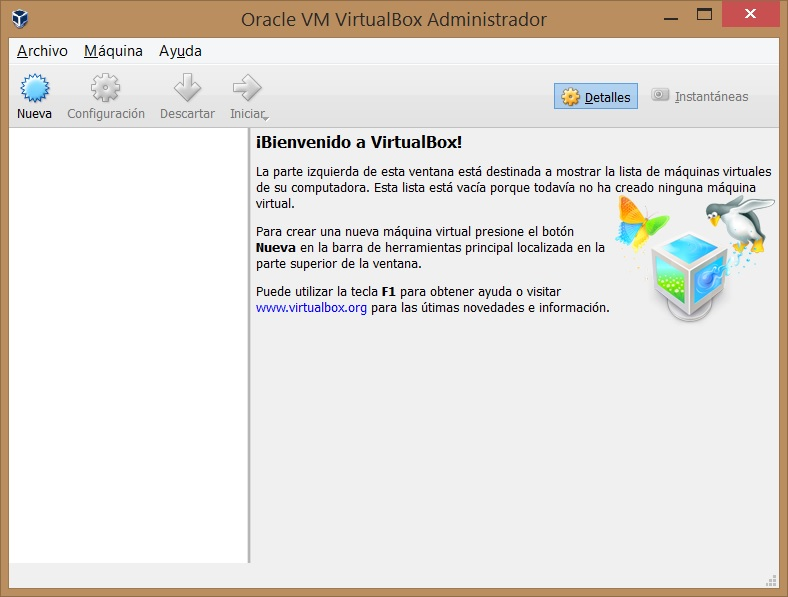
\includegraphics[width=0.7\linewidth]{figuras/vm-1}
	\caption{Virtual box - inicio}
	\label{fig:vm1}
\end{figure}

Le asignamos la memoria RAM a la máquina virtual 2048 MB es el mínimo recomendado, yo he usado 4.096 MB. Seleccionamos la opción \textit{Crear un disco duro virtual ahora}, ya que no tenemos ninguno creado anteriormente y hacemos clic en \underline{Crear} y seleccionamos en la siguiente pantalla la opción VDI (Virtual BOX Disk Image) y con tamaño “Reservado Dinámico” para que ocupe lo que realmente necesite.

\begin{figure}[H]
	\centering
	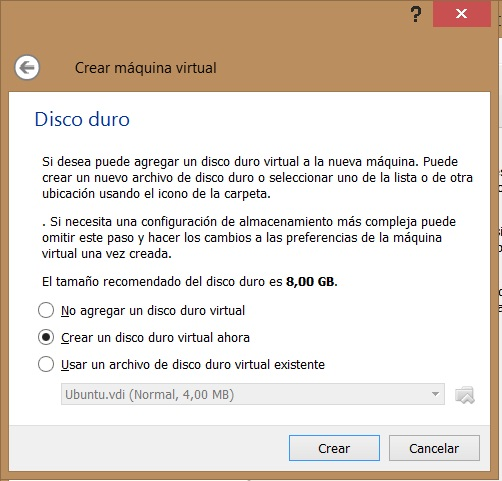
\includegraphics[width=0.5\linewidth]{figuras/vm-2}
	\caption{Virtual box - crear disco duro}
	\label{fig:vm2}
\end{figure}

Ya tenemos creada la máquina virtual. Solo nos queda empezar a instalar Ubuntu en el siguiente apartado.

\begin{figure}[H]
	\centering
	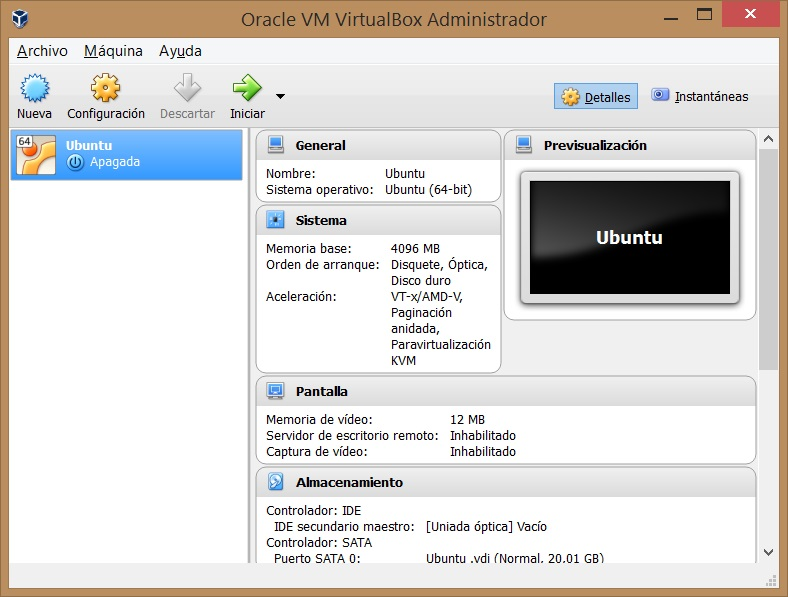
\includegraphics[width=0.6\linewidth]{figuras/vm-3}
	\caption{Virtual box-vm creada}
	\label{fig:vm3}
\end{figure}

Pulsamos sobre \textit{iniciar} para arrancar la máquina virtual y empezar la instalación de Ubuntu, nos pedirá que seleccionemos la imagen ISO que hemos descargado anteriormente. La instalación comienza con un asistente de instalación en el que debemos seleccionar el idioma a usar y pulsar en “instalar Ubuntu”. Su instalación ha sido bastante rápida, nos ha llevado un total de 9 minutos.

\begin{figure}[H]
	\centering
	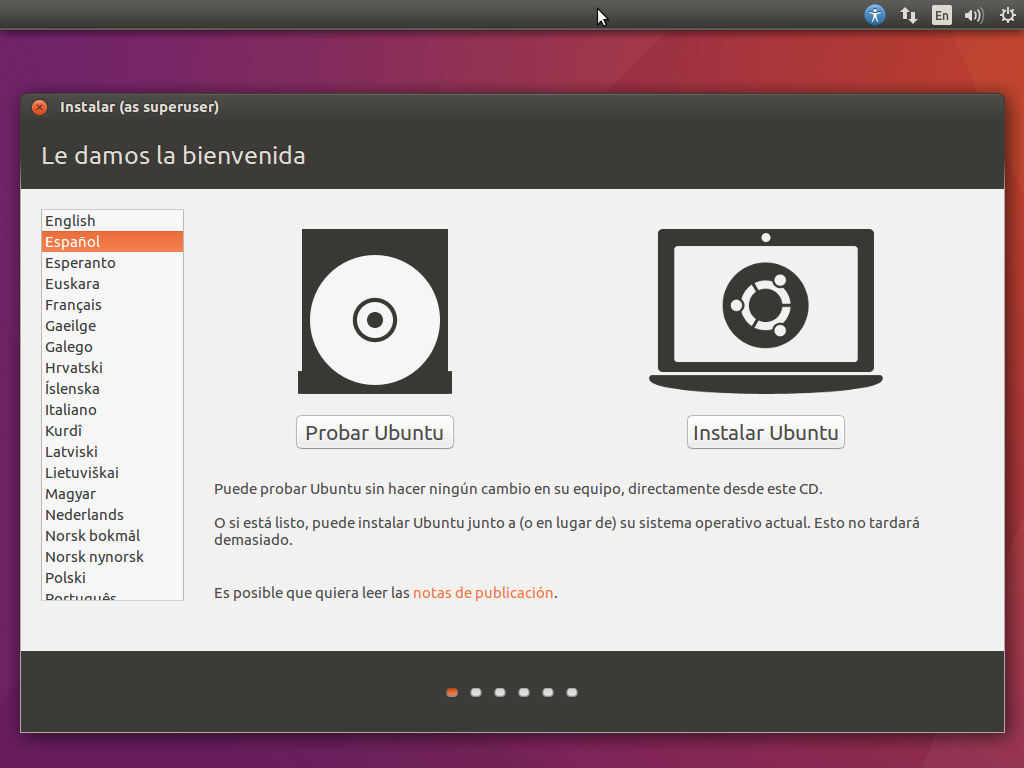
\includegraphics[width=0.7\linewidth]{figuras/vm-4}
	\caption{Instalación ubuntu}
	\label{fig:vm4}
\end{figure}

En la siguiente pantalla nos da la opción de descargar las actualizaciones e instalar software de terceros para reproducir archivos multimedia y otros. A continuación, nos saldrá el asistente del particionado del disco duro, en este caso vamos a usar todo el disco virtual que hemos creado por lo que dejamos la opción por defecto y pulsamos en \textit{instalar ahora}
Configuramos las particiones por defecto, seleccionamos nuestra zona horaria y pulsamos en \textit{continuar}, y elegimos nuestra distribución del teclado y \textit{continuar}. Luego nos saldrá una última pantalla en la que deberemos poner nuestro nombre de usuario y contraseña. También podemos seleccionar la opción de inicio de sesión automático.

\begin{figure}[H]
	\centering
	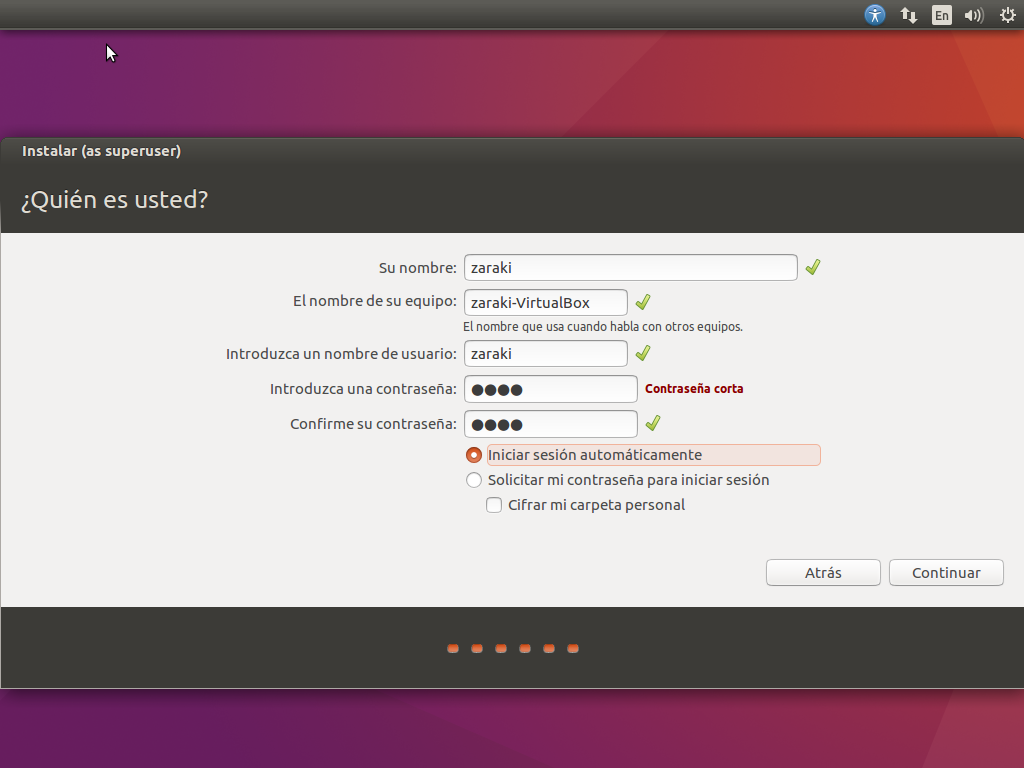
\includegraphics[width=0.8\linewidth]{figuras/vm-5}
	\caption{Instalación ubuntu - usuario y password}
	\label{fig:vm5}
\end{figure}

Finalmente reiniciamos nuestro sistema y ya tendremos un Ubuntu 16.04 LTS funcionando.

\subsection{Instalar Eclipse}
Instalar el JDK de Oracle
En un principio debemos verificar si disponemos de una versión de desarrollo de java instalada. Se detallan los comandos para verificar instalar en modo consola.

\begin{lstlisting}

java -version
sudo apt-get update
sudo apt-get install python-software-properties
sudo add-apt-repository ppa:webupd8team/java
sudo apt-get install oracle-java8-installer
\end{lstlisting}

Una Vez instalada se puede comprobar la instalación.

\begin{figure}[H]
	\centering
	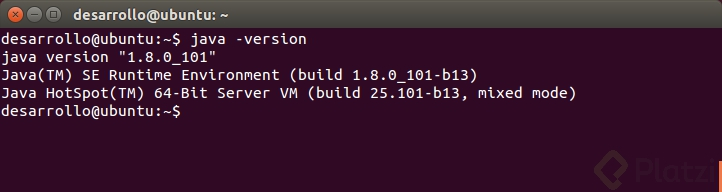
\includegraphics[width=0.7\linewidth]{figuras/ecli-1}
	\caption{Terminal ubuntu}
	\label{fig:ecli1}
\end{figure}

Descargar e Instalar Eclipse Oxigen
Ir a la página oficial y descargar la última versión para Linux 64 bits. Se extrae el archivo de la carpeta y se mueve la carpeta a otra ubicación más cómoda.

\begin{lstlisting}

sudo mkdir -p /opt/ide/64
sudo mv ~/Downloads/eclipse /opt/ide/64
cd /opt/ide/64
sudo chown -R root:root eclipse
sudo ln -sf /opt/ide/64/eclipse/eclipse /usr/bin/

\end{lstlisting}

\begin{figure}[H]
	\centering
	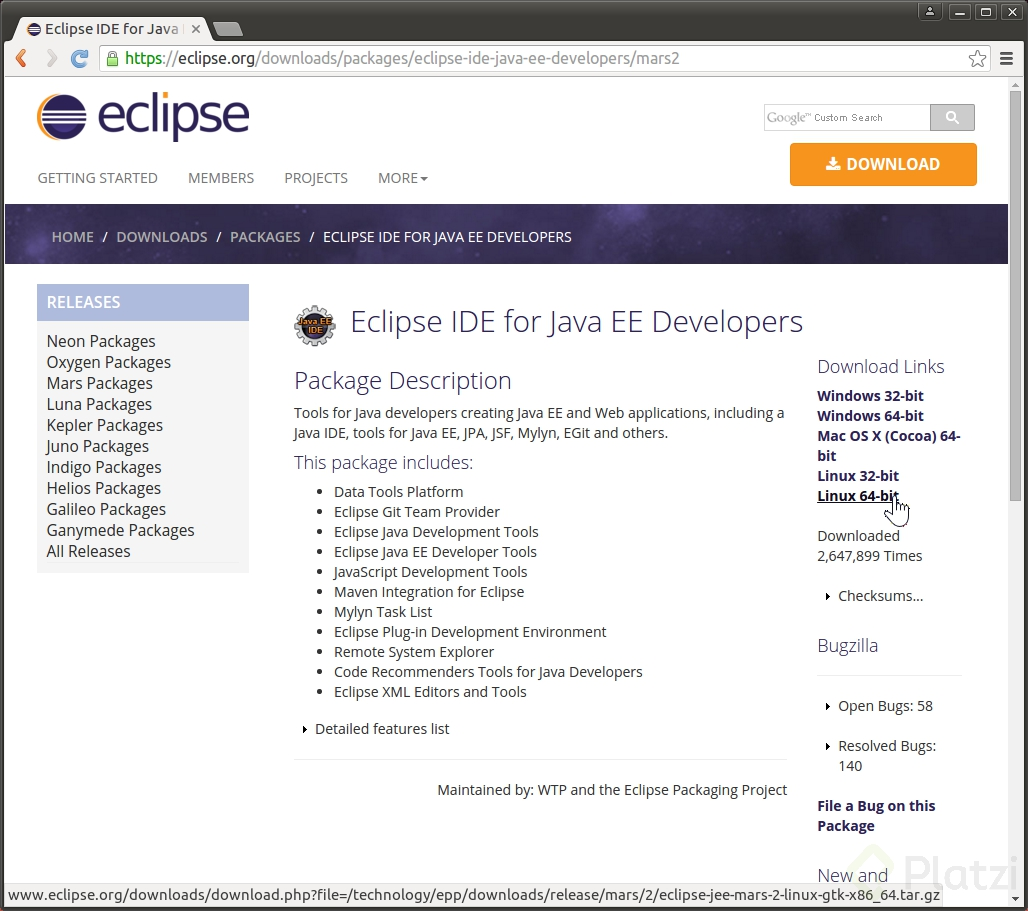
\includegraphics[width=0.6\linewidth]{figuras/ecli-2}
	\caption{Ventana Eclipse}
	\label{fig:ecli2}
\end{figure}


Definir Eclipse como un programa para su acceso directo
Se ejecuta el siguiente comando, lo cual abrirá una carpeta dónde se encuentran las aplicaciones del sistema con todos los permisos para administrarlos.

\begin{lstlisting}

sudo nautilus /usr/share/applications
\end{lstlisting}

Para generar un acceso directo a eclipse. Eclipse.desktop

\begin{lstlisting}

sudo mv /usr/share/applications/Eclipse.desktop /usr/share/applications/eclipse-mars-2.desktop
sudo gedit /usr/share/applications/eclipse-mars-2.desktop
[Desktop Entry]
Name=Eclipse Mars 2
Comment=IDE for Java
Exec=/usr/bin/eclipse
Icon=/opt/ide/64/eclipse/icon.xpm
Terminal=false
StartupNotify=true
Version=2.0
Type=Application
Categories=Development;Utility;
\end{lstlisting}

\subsection{Instalar Android studio}
Descarga de Android Studio de su página principal, Hacemos click sobre \textit{Download Android Studio} y comenzará la descarga. Nos descargará un fichero comprimido el cual debemos colocar sobre el directorio desde el que queramos ejecutarlo.
Instalación de Android Studio
Una vez descomprimido el archivo podremos ver una carpeta similar a la siguiente. Debemos acceder a la carpeta android-studio/bin y ejecutar el script llamado studio.sh para arrancar el programa.

\begin{figure}[H]
	\centering
	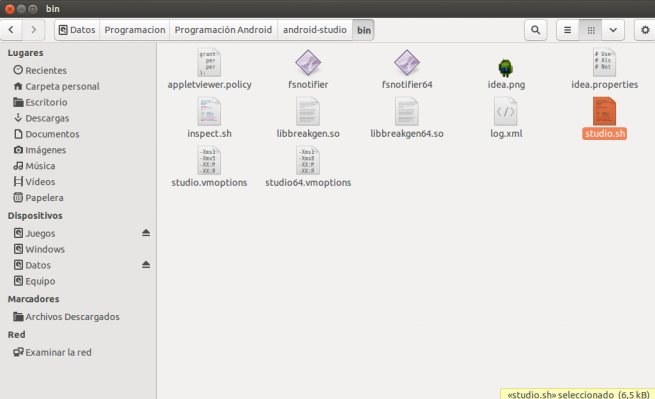
\includegraphics[width=0.6\linewidth]{figuras/and-1}
	\caption{Archivador ubuntu}
	\label{fig:and1}
\end{figure}


Seleccionaremos \textit{New project} para crear un nuevo proyecto desde el que podremos comenzar a utilizar la nueva IDE. Una vez finalizamos el asistente de inicio ya podremos ver la interfaz del programa.

\begin{figure}[H]
	\centering
	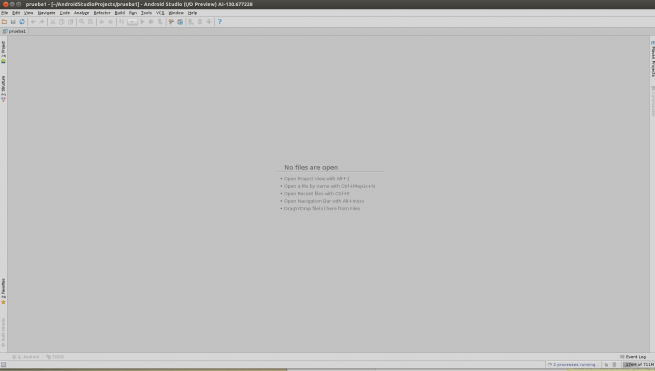
\includegraphics[width=0.7\linewidth]{figuras/and-2}
	\caption{Android studio}
	\label{fig:and2}
\end{figure}

En caso de tener proyectos ya creados o empezados con Eclipse podemos importarlos de forma muy sencilla. Para ello debemos situarnos sobre el \textit{menú file – import} y seleccionar el proyecto que queremos importar. Una vez allí seleccionaremos la opción \textit{Create project from existing sources} y ya tendremos nuestro proyecto importado en nuestro nuevo IDE para continuar desarrollando desde él. Podemos ver que la interfaz de la nueva IDE es bastante simple y sencilla de utilizar.

\begin{figure}[H]
	\centering
	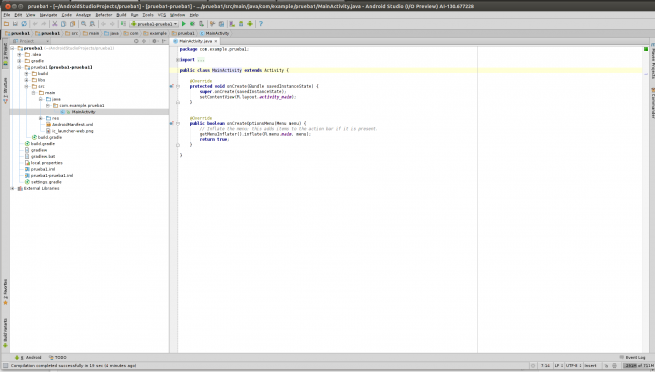
\includegraphics[width=0.7\linewidth]{figuras/and-3}
	\caption{Android studio - ejemplo de proyecto }
	\label{fig:and3}
\end{figure}

\pagebreak

Para crear un lanzador Primero abrimos la consola y digitamos lo siguiente:
\begin{lstlisting}
sudo gedit /usr/share/applications/eclipse.desktop
\end{lstlisting}

Esto obviamente abrirá el gedit y en el ingresamos:

\begin{lstlisting}

[Desktop Entry]
Name=Android Studio
Comment=Android Studio IDE
Exec=/home/tu_usuario/android-studio/bin/studio.sh
Icon=/home/tu_usuario/android-studio/bin/idea.png
Terminal=false
Type=Application

\end{lstlisting}

\subsection{Instalar Xamp}
Descarga el instalador de XAMPP. Puedes conseguirlo en apachefriends.org/download.html. Asegúrate de descargar la versión correcta para tu sistema (32 o 64 bits). En esta guía se utilizará como ejemplo la versión 5.6.3 de 64 bits. Asegúrate de cambiar los comandos según la versión que vayas a instalar.
Abre la Terminal. Antes de poder instalar XAMPP, necesitarás cambiar los permisos de modo que puedas ejecutar el archivo que descargaste. 
Cambia los permisos. Ingresa el siguiente comando y presiona Enter, escribiendo también tu contraseña de ser necesario: 

\begin{lstlisting}

sudo chmod +x xampp-linux-x64-5.6.3-0-installer.run
\end{lstlisting}

Puedes arrastrar el archivo descargado hacia la ventana de la Terminal para ingresar el nombre y la ubicación del archivo en forma automática.
Ejecuta el instalador. Después de cambiar los permisos, podrás ejecutar el instalador para comenzar a instalar XAMPP. Escribe el siguiente comando y presiona Enter: 

\begin{lstlisting}

sudo ./xampp-linux-x64-5.6.3-0-installer.run
\end{lstlisting}

Sigue las instrucciones para instalar XAMPP. Se abrirá el instalador gráfico para guiarte a través del resto del proceso de instalación. En la mayoría de los casos, es mejor dejar todas las opciones con su configuración predeterminada.
\subsection{Instalar Tomcat}
Instalamos Tomcat  en modo terminal.

\begin{lstlisting}

sudo apt-get install tomcat8
\end{lstlisting}

Editamos el archivo de configuración del bash:

\begin{lstlisting}

sudo nano ~/.bashrc
export JAVA_HOME=/usr/lib/jvm/default-java
export CATALINA_HOME=/var/lib/tomcat7
\end{lstlisting}

Por último nos quedaría modificar el archivo de usuarios:

\begin{lstlisting}

sudo nano /var/lib/tomcat7/conf/tomcat-users.xml
Deberemos dejarlo parecido a:
<tomcat-users>
<role rolename="admin-gui"/>
<role rolename="admin-script"/>
<role rolename="manager-gui"/>
<role rolename="manager-status"/>
<role rolename="manager-script"/>
<role rolename="manager-jmx"/>
<user username="admin" password="1234" roles="standard,manager-gui,manager-status,manager-script,manager-jmx,admin-gui,admin-script" />
</tomcat-users>
\end{lstlisting}

Por último, sólo tendríamos que reiniciar el servicio de Tomcat (sudo service tomcat8 restart) y ya podríamos acceder a nuestro Tomcat desde cualquier navegador poniendo la siguiente ruta: localhost:8080 En la que nos aparecerá el archivo por defecto con unos enlaces a los ejemplos, documentación, etc…

Si hemos instalado también el paquete de administración, podremos de una manera sencilla ver, cambiar y desplegar nuestras aplicaciones Java, desde http://local-host: 8080/manager/html introduciendo el usuario y la contraseña que hayamos puesto en el archivo de configuración.


\begin{figure}[H]
	\centering
	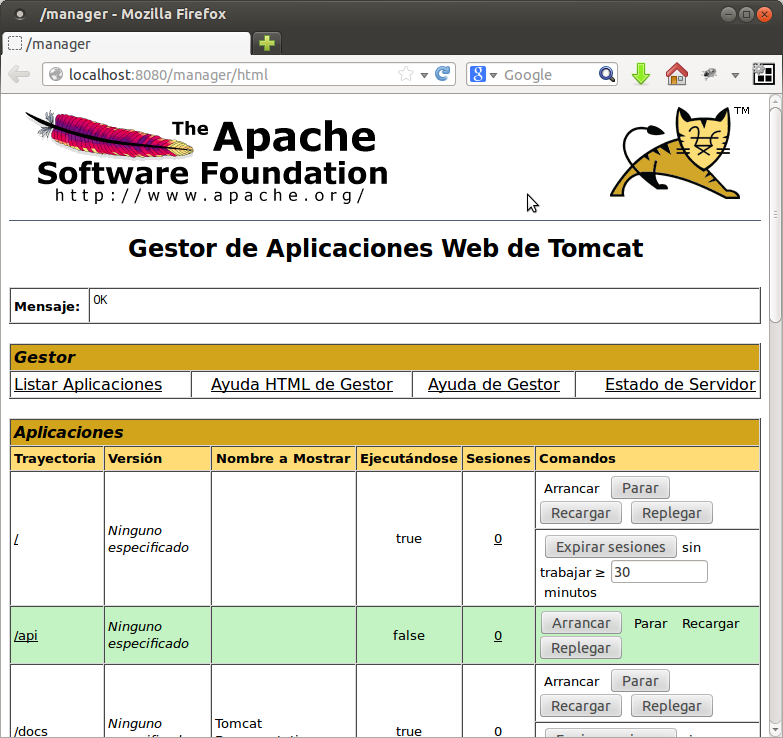
\includegraphics[width=0.8\linewidth]{figuras/apache}
	\caption{Tomcat Manager}
	\label{fig:apache}
\end{figure}


\chapter{ANEXO IV}

\section{Configuracion de los proyectos cliente y servidor}

\subsection{Creación del proyecto web service}

Una vez arrancado el entorno Eclipse, vamos a crear un proyecto nuevo (en el menu Archivo -> Nuevo -> Dynamic Web Project.), donde definiremos el nombre de nuestro proyecto, el runtime al que se destina nuestro proyecto, en este caso al servidor tomcat que instalamos en nuestro sistema. Después agregamos al proyecto las librerias de JAX-RS a nuestro proyecto en el boton de “configurar” – “Modificar”.

\begin{figure}[H]
	\centering
	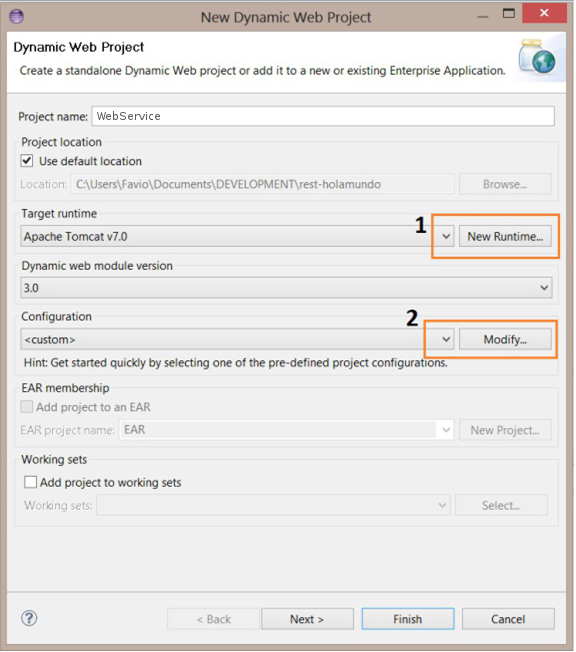
\includegraphics[width=0.4\linewidth]{figuras/service-1}
	\caption{WebService - creación}
	\label{fig:ws1}
\end{figure}

En el directorio src de nuestro proyecto agregamos la siguiente clase “LoggerWS”, dentro del paquete com.group.six:

\begin{lstlisting}[style=JAVA]
package com.intraza.rest;

import javax.ws.rs.Consumes;
import javax.ws.rs.GET;
import javax.ws.rs.POST;
import javax.ws.rs.Path;
import javax.ws.rs.Produces;
import javax.ws.rs.QueryParam;
import javax.ws.rs.core.MediaType;

import org.apache.log4j.Logger;
import org.codehaus.jackson.map.ObjectMapper;

import com.intraza.rest.db.*;
import com.intraza.rest.db.datos.*;

@Path(value = "/sincroniza")
public class InTrazaWS {
	
	private static Logger logger = Logger.getLogger(InTrazaWS.class);
	
	@GET
	@Path("articulos")
	@Produces(MediaType.APPLICATION_JSON)
	public List<Articulo> consultaArticulosBD() {
		return JDBCQuery.getArticulos();
	}
	
	..............
	
	@POST
	@Path("prepedido")
	@Consumes(MediaType.APPLICATION_JSON)
	@Produces(MediaType.APPLICATION_JSON)
	public ResultadoEnvioPedido enviaPrepedidoBD(String jsonPrepedido) {
		ResultadoEnvioPedido resultadoEnvio = null;
		try {
			// Convertimos el JSON que nos llega a un objeto java
			ObjectMapper mapper = new ObjectMapper();
			JsonPedido datosPrepedido = mapper.readValue(jsonPrepedido, JsonPedido.class);
			
			logger.debug("##### observaciones (" + datosPrepedido.getObservaciones() + ") ######");
			
			resultadoEnvio = JDBCQuery.postPrepedido(datosPrepedido);
		} catch (Exception e) {
			resultadoEnvio = new ResultadoEnvioPedido(ResultadoEnvioPedido.CON_ERROR,
			"Se ha producido una excepcion al decodificar JSON (" + jsonPrepedido + ") (" + e.toString() + ")");
		}
		
		return resultadoEnvio;
	}
\end{lstlisting}

Ahora es necesario agregar al archivo web.xml, que eclipse nos genero sobre el directorio WEB-INF de nuestro proyecto, la configuración de Jersey, y el servlet mapping que es la ruta donde se invocara a nuestro servicio, el archivo queda asi:
\begin{lstlisting}[style=JAVA]
<?xml version="1.0" encoding="UTF-8"?>
<web-app xmlns:xsi="http://www.w3.org/2001/XMLSchema-instance"
xmlns="http://java.sun.com/xml/ns/javaee"
xsi:schemaLocation="http://java.sun.com/xml/ns/javaee http://java.sun.com/xml/ns/javaee/web-app_3_0.xsd"
id="WebApp_ID" version="3.0">
<display-name>InTrazaWeb20</display-name>

<servlet>
	<servlet-name>IntrazaWeb</servlet-name>
	<servlet-class>com.sun.jersey.spi.container.servlet. ServletContainer</servlet-class>
	<init-param>
		<param-name>com.sun.jersey.config.property. packages</param-name>
		<param-value>com.intraza.rest</param-value>
	</init-param>
	<init-param>
		<param-name>com.sun.jersey.api.json. POJOMappingFeature</param-name>
		<param-value>true</param-value>
	</init-param>
	<load-on-startup>1</load-on-startup>
</servlet>
<servlet-mapping>
	<servlet-name>IntrazaWeb</servlet-name>
	<url-pattern>/rest/ *</url-pattern>
</servlet-mapping>

<welcome-file-list>
<welcome-file>index.jsp</welcome-file>
</welcome-file-list>
</web-app>
\end{lstlisting}

Para poder compilar y correr nuestro código es necesario antes agregar a nuestro proyecto la implementación Jersey a las librerías de nuestro proyecto, para ello hay que descargarlas del sitio de Jersey, aqui. Para después copiar los jar en el directorio WEB-INF/libs. Otra opción es convertir el proyecto a un proyecto maven, y usar las configuracion a traves del archivo pom.

Para visualizar nuestra aplicación, podemos publicar el servlet al dar Run as -> Run on server. Si aún no tenemos configurado nuestro servidor tomcat, el wizard nos guiara.

La URL donde encontraremos nuestro servicio esta construida de la siguiente manera: http://nuestroservidor:puerto/contextroot/servletmapping/class-path

\begin{itemize}
	\item Nuestroservidor: es el servidor al que publicamos nuestro servlet, con su puerto en el que funciona
	\item Contextroot: es generalmente el nombre de nuestro proyecto, en las propiedades de nuestro proyecto podemos cambiar esto
	\item Servletmapping: es la ruta que definimos en el archivo web.xml donde estaran nuestras clases.
	\item Class-path: es el nombre de la ruta que definimos en nuestra clase con @Path(“/class-path”)
\end{itemize}

\subsection{Integrar un cliente web service}

Por la propia particularidad del web service, un servicio REST, no necesitamos generar un cliente web especifico solo tenemos que tener en cuenta el empaquetado de datos y enviarlos a una url especifica del servicioWeb. Simplemente debemos incluir una clase que gestione la comunicacion. En el codigo siguiente se puede ver un ejemplo que envía al webService un Conjunto de datos a una url especifica.

\begin{lstlisting}[style=JAVA]

package com.six.group.listener.utils;

import android.os.StrictMode;

import com.fasterxml.jackson.databind.ObjectMapper;
import com.six.group.listener.data.json.Datos;

import java.io.BufferedReader;
import java.io.InputStream;
import java.io.InputStreamReader;
import java.io.OutputStream;
import java.net.HttpURLConnection;
import java.net.URL;

public class WebServicesUtils {
private static Integer sincro = 1800;
private static String urlWebServiceRest;


public WebServicesUtils(String puerto, String ip) {
urlWebServiceRest = "http://" + ip + ":" + puerto + "/WebService/enviar/";
}

public String invocaWebServiceHttp(final Datos datos, String action) throws Exception {

StrictMode.ThreadPolicy policy = new StrictMode.ThreadPolicy.Builder()
.detectAll()
.penaltyLog()
.build();
StrictMode.setThreadPolicy(policy);

String result = "";
String urlToInvocate = urlWebServiceRest + action;

System.out.println("Sincronizacion : TRAZA - URL (" + urlToInvocate + ") segundo timeout (" + sincro + ")");

final URL url = new URL(urlToInvocate);
final HttpURLConnection connection = (HttpURLConnection) url.openConnection();
connection.setConnectTimeout(sincro * 1000);
connection.setReadTimeout(sincro * 1000);
connection.setRequestMethod("POST");
connection.setDoOutput(true);
connection.setRequestProperty("Content-Type", "application/json");
final ObjectMapper mapper = new ObjectMapper();
final String jsonRequest = mapper.writeValueAsString(datos);
final OutputStream os = connection.getOutputStream();
os.write(jsonRequest.getBytes());
os.flush();
final InputStream content = connection.getInputStream();
final BufferedReader in = new BufferedReader(new InputStreamReader(content));
String line;
while (null != (line = in.readLine())) {
result += line;
}
return result;
}
}

\end{lstlisting}


\chapter{ANEXO V}

\section{Compilación de los proyectos}

\subsection{Compilación Android}

Lo primero que debemos hacer es abrir nuestro proyecto en Android Studio y asegurarnos de que no hay ningún error de código ni de compilación ya que, de lo contrario, no se completará la compilación.

Si todo está correcto (no tenemos nada marcado en rojo en el código) abriremos el menú \textit{Build} de la parte superior de la pantalla y veremos dos opciones:

\begin{itemize}
	\item Build APK
	\item Generate Signed APK
\end{itemize}	

La primera opción nos va a permitir generar un archivo apk para instalarlo en un dispositivo, pero el archivo no estará firmado. La segunda opción nos permitirá generar un archivo de forma (o utilizar uno existente) para firmar digitalmente nuestra aplicación. Esta opción es para  subir la app al google play.
En nuestro caso vamos a seleccionar directamente la segunda opción, la de generar el archivo APK firmado digitalmente. Pulsamos sobre ella y veremos una nueva ventana similar a la siguiente.

\begin{figure}[H]
	\centering
	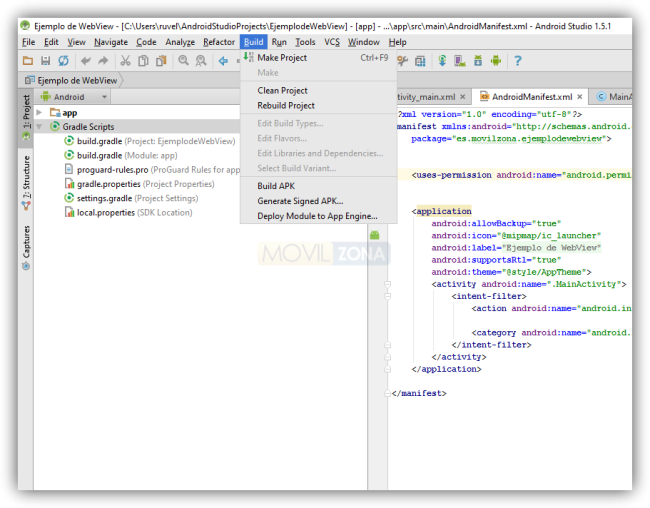
\includegraphics[width=0.7\linewidth]{figuras/build-1}
	\caption{Android studio-buid}
	\label{fig:bld1}
\end{figure}


Aquí podemos elegir dos opciones. Si ya tenemos una clave creada anteriormente la cargaremos desde el botón \textit{Choose Existing} e introduciremos el correspondiente nombre, usuario y contraseña para poder utilizarla. 

\begin{figure}[H]
	\centering
	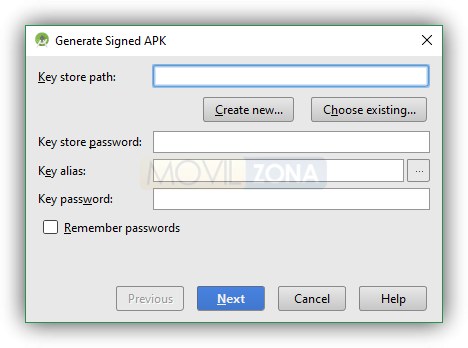
\includegraphics[width=0.6\linewidth]{figuras/build-2}
	\caption{Generar aplicación firmada - key}
	\label{fig:bld2}
\end{figure}

Si nunca hemos generado una clave o queremos crear una nueva por diversos motivos, pulsaremos sobre \textit{Create New}.
Se nos abrirá una nueva ventana como la siguiente:

\begin{figure}[H]
	\centering
	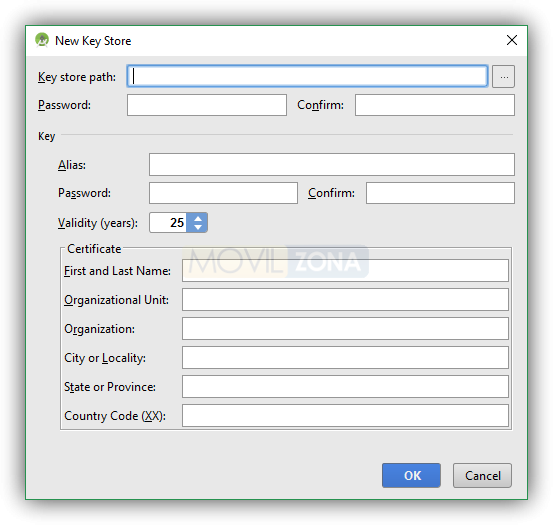
\includegraphics[width=0.6\linewidth]{figuras/build-3}
	\caption{Generar aplicación firmada - nuevo key store}
	\label{fig:bld3}
\end{figure}

En esta ventana debemos rellenar los siguientes apartados:

\begin{itemize}
	\item Key Store Path: Ruta donde guardaremos la clave.
	\item Password: Contraseña 1 para nuestra clave.
	\item Alias: Nombre que daremos a nuestra clave.
	\item Password: Contraseña 2 para nuestra clave.
	\item Validity: Tiendo de validez de la clave (en años).
	\item First and last name: Nombre y apellidos.
	\item Organizational Unit: Nombre de nuestra empresa.
	\item Organization: Nuestra empresa (otra vez)
	\item City: Ciudad.
	\item State: Estado, país.
	\item Country Code: Código de nuestro país.
\end{itemize}


Aceptamos y Android Studio guardará el fichero de la clave en la ruta especificada. Debemos guardar a buen recaudo este archivo ya que sin él perderemos el control sobre nuestra aplicación y no podremos actualizarla más adelante. Una copia de seguridad en un USB y en la nube (cifrada, para evitar robos) es la mejor opción.
Una vez hecho esto, Android Studio cargará automáticamente nuestra clave generada y nos permitirá seguir con la generación del apk.


\begin{figure}[H]
	\centering
	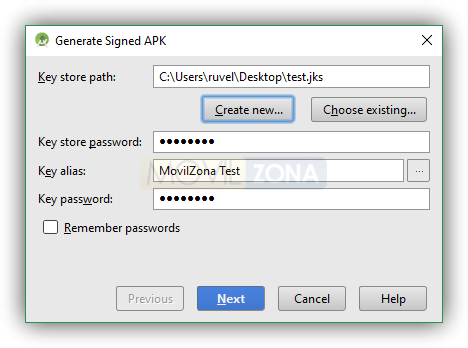
\includegraphics[width=0.6\linewidth]{figuras/build-4}
	\caption{Generar aplicación firmada- key creada}
	\label{fig:bld2}
\end{figure}


Pulsamos \textit{Next} y en el siguiente paso nos preguntará la ruta donde guardará el APK y el tipo de compilación que va a ser (release para publicar o debug para probar y depurar).

Pulsamos sobre Finish y listo. Android Studio compilará nuestra aplicación y la guardará en la ruta especificada. Una vez finalice el proceso veremos un aviso en el IDE que no indica que todas las tareas se han realizado correctamente.

\begin{figure}[H]
	\centering
	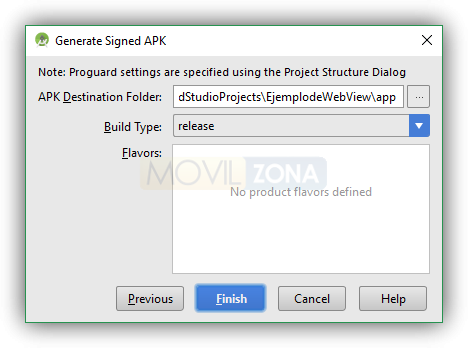
\includegraphics[width=0.6\linewidth]{figuras/build-5}
	\caption{Generar aplicacion firmada - finalizar}
	\label{fig:bld2}
\end{figure}

\subsection{Compilación Eclipse}

Para la compilación en eclipse utilizamos Maven. Este ya nos proporciona un WAR generado cuando ejecutamos sus comandos. Pulsamos con el botón derecho sobre el proyecto para elegir “Run As”. En el desplegable podremos comprobar como hay ya varios comandos pre-configurados por el plugin de Maven en Eclipse; es decir, que pulsando un botón ejecutaremos estos comandos sin tener que escribir una palabra en la línea de comandos.

\begin{figure}[H]
	\centering
	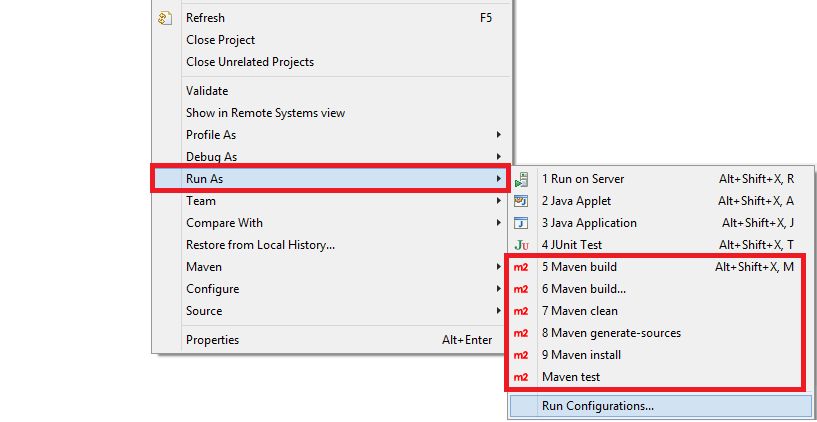
\includegraphics[width=0.5\linewidth]{figuras/maven/maven1}
	\caption{Eclipse - opciones maven}
	\label{fig:mvn1}
\end{figure}

\subsubsection{POM}

El archivo descriptivo que contendrá las opciones de compilación, dependencias, etc, es el “pom.xml”, el de resto de pestañas son asistentes para configurar el POM de una manera más sencilla, que aquí no entraremos pero échalas un vistazo que son útiles.

\begin{figure}[H]
	\centering
	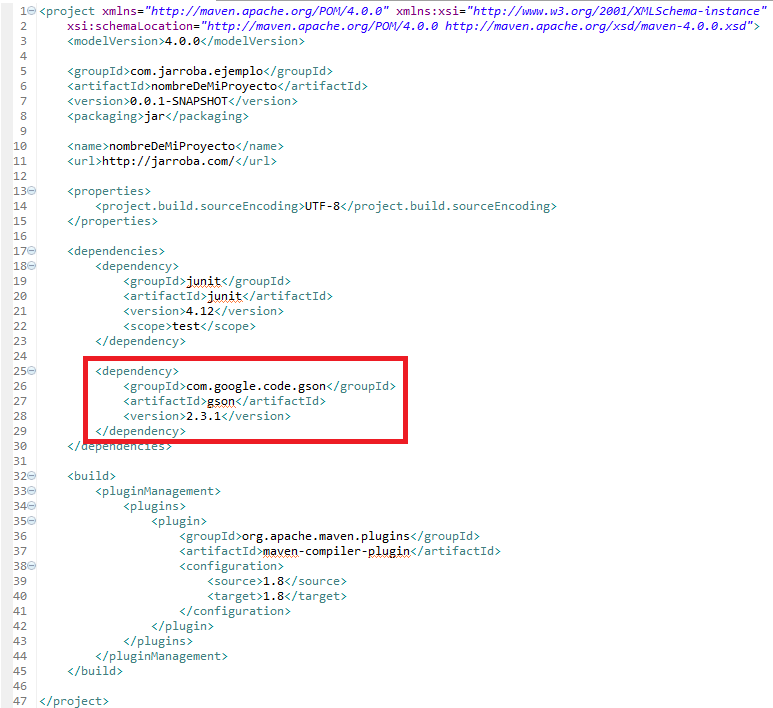
\includegraphics[width=0.5\linewidth]{figuras/maven/maven2}
	\caption{Eclipse - pom.xml}
	\label{fig:mvn2}
\end{figure}

Podemos describir su estructura básica con el siguiente listado:

\begin{itemize}
	\item \textbf{build:} Se ocupa de declarar la estructura del proyecto, gestionar plugins, y configura los informes.
	\item \textbf{properties:} Propiedades y/o variables para maven.
	\item \textbf{pluginManagement:} Solo configura los plugins que son referenciados dentro de elementos de los plugins de los hijos (plugins).
	\item \textbf{plugins:} Los plugins nos aportan funcionalidades extra.
	\begin{itemize}
		\item \textbf{groupId,artifactId, version}
		\item \textbf{extensions,inherited, configuration}
		\item \textbf{dependencies} 
	\end{itemize}
	\item \textbf{dependencies:} Son las dependencias (bibliotecas) que sean necesarias para la ejecución de la aplicación.
\end{itemize}

\subsubsection{Run options}

Por mediación del comando “maven install” construiremos un war completamente funcional y desplegable en tomcat. 

\begin{figure}[H]
	\centering
	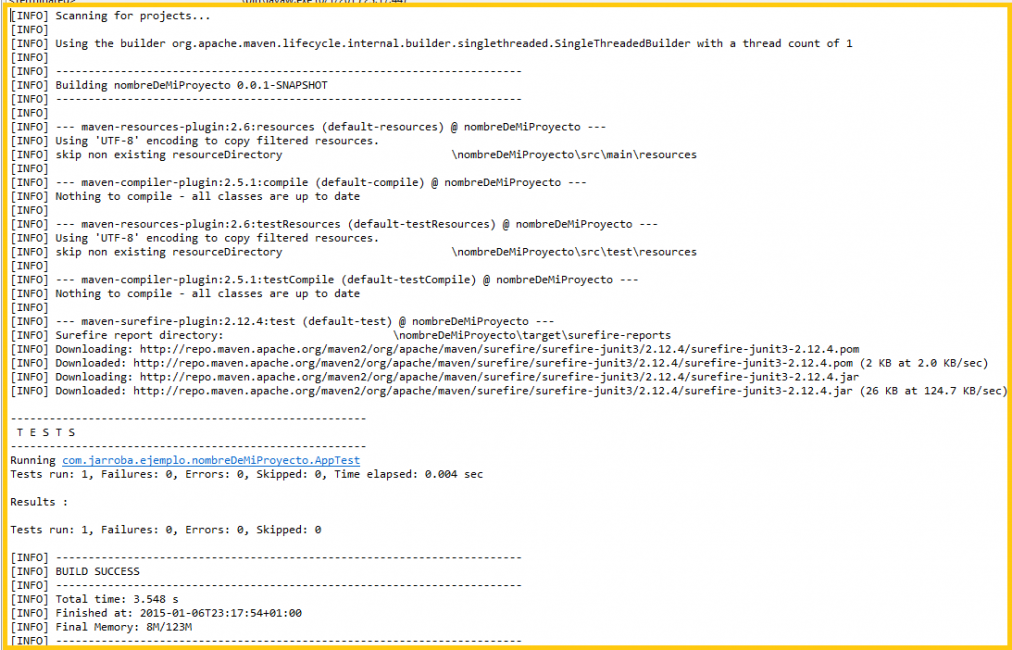
\includegraphics[width=0.7\linewidth]{figuras/maven/maven3}
	\caption{Eclipse - salida de consola maven}
	\label{fig:mvn3}
\end{figure}


